\subsection{Oudit onderdeel}

Die oudit onderdeel is verantwoordelik vir die monitering en logboekhouding
van alle gebruikers- en transaksie-aktiwiteite in die stelsel. Dit sluit die
logboekhouding van gebruikersgebeurtenisse, transaksie-oudit, en die
verskaffing van toegang tot oudit-inligting vir administrateurs in. Hierdie
onderdeel is kritiek vir sekuriteit, nakoming van regulasies, en
foutoplossing.

\begin{figure}[H]
    \centering
    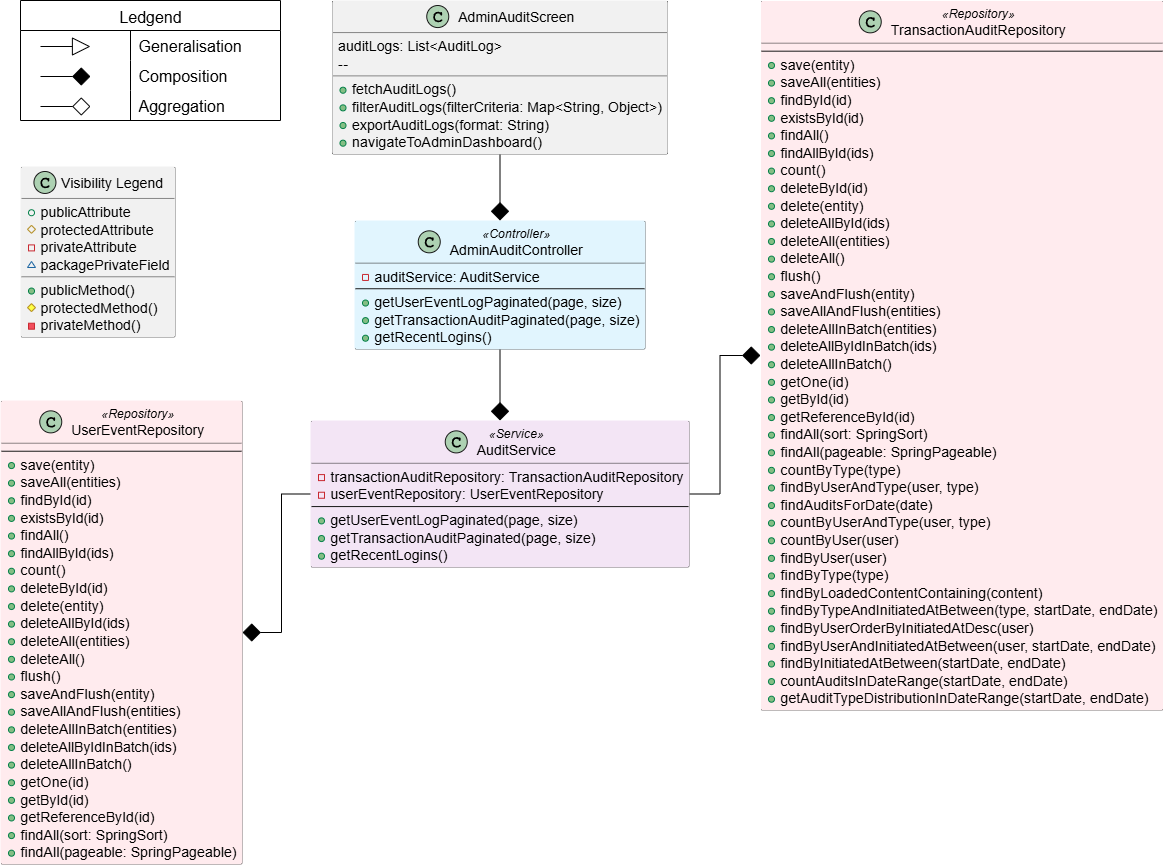
\includegraphics[width=\textwidth]{figures/class_diagrams/audit-subsystem.png}
    \caption{Oudit onderdeel klasdiagram}
    \label{fig:audit_subsystem_class_diagram}
\end{figure}

Hier volg die CRC kaarte vir die belangrikste klasse in hierdie
onderdeel.

\vspace{1em}
\textbf{AdminAuditScreen} bied administrateurs 'n oorsig van oudit-logboeke, met die vermoë om te filter en uit te voer in verskillende formate.
\begin{table}[H]
\centering
\begin{tabular}{|p{0.4\textwidth}|p{0.4\textwidth}|}
    \hline
    \multicolumn{2}{|c|}{\textbf{AdminAuditScreen}} \\
    \hline
    \textbf{Verantwoordelikhede} & \textbf{Medewerkers} \\
    \hline
    Wys oudit-logboeke \newline
    Filter oudit-logboeke volgens kriteria \newline
    Voer oudit-logboeke uit in verskillende formate
    &
    AdminAuditController \\
    \hline
\end{tabular}
\caption{CRC vir AdminAuditScreen}
\label{tab:crc_admin_audit_screen}
\end{table}
\vspace{1em}

\textbf{AdminAuditController} hanteer versoeke vanaf die administrateur se ouditkoppelvlak en verskaf toegang tot relevante ouditdata.
\begin{table}[H]
\centering
\begin{tabular}{|p{0.4\textwidth}|p{0.4\textwidth}|}
    \hline
    \multicolumn{2}{|c|}{\textbf{AdminAuditController}} \\
    \hline
    \textbf{Verantwoordelikhede} & \textbf{Medewerkers} \\
    \hline
    Hanteer oudit-versoeke van administrateurs \newline
    Verskaf toegang tot gebruikersgebeurtenisse \newline
    Verskaf toegang tot transaksie-oudit log
    &
    AuditService \\
    \hline
\end{tabular}
\caption{CRC vir AdminAuditController}
\label{tab:crc_admin_audit_controller}
\end{table}
\vspace{1em}

\textbf{AuditService} in die dienslaag verwerk ouditdata, verskaf resultate en onlangse aanmeldings, en tree op as dienslaag vir ouditlogika.
\begin{table}[H]
\centering
\begin{tabular}{|p{0.4\textwidth}|p{0.4\textwidth}|}
    \hline
    \multicolumn{2}{|c|}{\textbf{AuditService}} \\
    \hline
    \textbf{Verantwoordelikhede} & \textbf{Medewerkers} \\
    \hline
    Verwerk oudit-logboeke \newline
    Verskaf gebruikersgebeurtenisse \newline
    Verskaf transaksie-oudit \newline
    Verkry onlangse aanmeldings
    &
    TransactionAuditRepository \newline
    UserEventRepository \\
    \hline
\end{tabular}
\caption{CRC vir AuditService}
\label{tab:crc_audit_service}
\end{table}

